\usetikzlibrary{calc,arrows.meta}
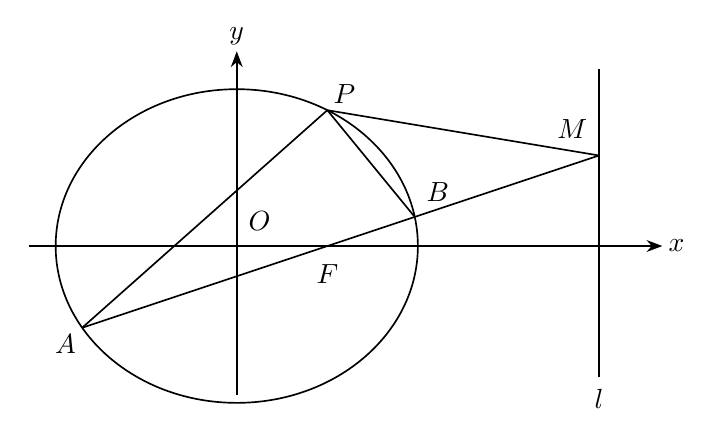
\begin{tikzpicture}[x=1.15cm,y=1.15cm,line width=.6pt,>=Stealth,font=\normalsize]
\coordinate (O) at (0,0);
\coordinate (P) at (1,1.5);
\coordinate (F) at (1,0);
\coordinate (A) at (-1.7071,-0.9024);
\coordinate (B) at (1.9652,0.3217);
\coordinate (M) at (4,1);
\coordinate (l1) at (4,-1.45);
\coordinate (l2) at (4,1.95);
\draw[->] (-2.3,0)--(4.7,0) node[anchor=west,inner sep=0pt,xshift=2pt] {$x$};
\draw[->] (0,-1.65)--(0,2.15) node[anchor=south,inner sep=0pt,yshift=2pt] {$y$};
\draw (O) ellipse [x radius=2, y radius=1.7320508];
\draw (A)--(M);
\draw (P)--(M);
\draw (P)--(A);
\draw (P)--(B);
\draw (l1)--(l2);
\node[anchor=south west,inner sep=2pt] at ($(O)+(0.06,0.10)$) {$O$};
\node[anchor=south west,inner sep=0pt,xshift=2pt,yshift=2pt] at (P) {$P$};
\node[anchor=north,inner sep=2pt] at ($(F)+(0,-0.14)$) {$F$};
\node[anchor=north east,inner sep=0pt,xshift=-2pt,yshift=-2pt] at (A) {$A$};
\node[anchor=south west,inner sep=2pt] at ($(B)+(0.06,0.10)$) {$B$};
\node[anchor=south east,inner sep=2pt] at ($(M)+(-0.06,0.12)$) {$M$};
\node[anchor=north,inner sep=2pt] at ($(l1)+(0,-0.06)$) {$l$};
\end{tikzpicture}
